\chapter{Körper}

Das Ziel dieses Kapitels ist es die Konzepte, beziehungsweise das Verhalten, von \\ Körpererweiterungen zu verstehen, beispielsweise von $\mathbb{R}$ auf $\mathbb{C}$, oder von $\mathbb{Q}$ auf $\mathbb{R}$. Weiters soll versucht werden alle endlichen Körper vollständig zu klassifizieren.

\section{Einführung}

\notedate{01.03.2023}
Zu Beginn wird der Begriff einer allgemeinen (oder auch universellen) Algebra definiert und es werden weiter einige spezielle Algebren vorgestellt.

\begin{definition}\label{def:algebra}\label{def:allg_algebra}
    Seien $A$ eine beliebige Menge, $\tau = (n_i)_{i \in I}$ eine Familie aus $\mathbb{N}_0$ über einer beliebigen Indexmenge $I$ und $(f_i)_{i \in I}$ eine Familie von Funktionen, wobei $f_i: A^{n_i} \to A$ ist. 
    Das Tupel $\mathfrak{A} = (A, (f_i)_{i \in I})$ heißt dann \emph{(allgemeine) Algebra}\index{Algebra!allgemeine} vom \emph{Typ}\index{Algebra!Typ} $\tau$. Die einzelnen Funktionen $f_i$ nennt man \emph{fundamentale Operationen}\index{fundamentale Operation} und haben \emph{Stelligkeit}\index{Stelligkeit} oder auch \emph{Arität}\index{Arität} $n_i$.
\end{definition}

\begin{remark}
    Für eine endliche Indexmenge $I = \{1, \ldots, m\}$ wird der Typ auch als $m$-Tupel $\tau = (n_1, \ldots, n_m)$ geschrieben und die Algebra als $\mathfrak{A} = (A, f_1, \ldots, f_m)$.
\end{remark}

\begin{remark}
    Eine nullstellige Operation $f_i$ bildet von der Menge $A^0 := \{\emptyset\}$ auf $A$ ab. Es ist also $f_i$ konstant mit $f(\emptyset) = a \in A$. Im Folgenden wird bei $n_i = 0$ nicht zwischen der Operation $f_i$ und dem Element $a$, auf das abgebildet wird, unterschieden.
\end{remark}

\begin{definition}\label{def:halbgruppe}
    Eine Algebra $\mathfrak{A} = (A, +)$ vom Typ $\tau = (2)$ heißt \emph{Halbgruppe}\index{Halbgruppe}, wenn 
    \begin{itemize}[topsep=0pt, label={--}]
        \item $\forall x,y,z \in A: (x + y) + z = x + (y + z)$ \tab (\emph{Assoziativität}\index{Assoziativität} von $+$)
    \end{itemize}
    gilt.
\end{definition}

\begin{example} $(\mathbb{R}, +), (\mathbb{R}, \cdot), (\mathbb{R}^{2\times 2}, \cdot), (\mathbb{N}, +)$ sind Halbgruppen.
\end{example}

\begin{definition}\label{def:monoid}
    Eine Algebra $\mathfrak{A} = (A, +, e)$ vom Typ $\tau = (2,0)$ heißt \emph{Monoid}\index{Monoid}, wenn
    \begin{itemize}[topsep=0pt, label={--}]
        \item $(A, +)$ eine Halbgruppe ist und
        \item $\forall x \in A: e + x = x + e = x$ \tab ($e$ ist \emph{neutrales Element}\index{neutrales Element} bezüglich $+$)
    \end{itemize}
    gilt.
\end{definition}

\begin{example}
    $(\mathbb{R}, +, 0), (\mathbb{R}, \cdot, 1), (\mathbb{R}^{2\times 2}, \cdot, E_2), (\mathbb{N}, \cdot, 1)$ sind Monoide.
\end{example}

\begin{definition}\label{def:gruppe}
    Eine Algebra $\mathfrak{A} = (A, +, e, -)$ vom Typ $\tau = (2,0,1)$ heißt \emph{Gruppe}\index{Gruppe}, wenn
    \begin{itemize}[topsep=0pt, label={--}]
        \item $(A, +, e)$ ein Monoid ist und
        \item $\forall x \in A: x + (-x) = (-x) + x = e$ \tab ($-$ bildet ab auf \emph{inverse Elemente}\index{invers!inverses Element})
    \end{itemize}
    gilt.
\end{definition}

\begin{example}
    $(\mathbb{R},+, 0, -), (\mathbb{Z}, +, 0, -)$ sind Gruppen.
\end{example}

\begin{remark}\label{rem:alternativegruppe}
    Manchmal werden Gruppen auch als Algebra $\mathfrak{A} = (A, +)$ vom Typ $\tau = (2)$ definiert, für die
    \begin{itemize}[topsep=0pt, label={--}]
        \item $\forall x,y,z \in A: (x + y) + z = x + (y + z)$,
        \item $\exists e \in A \forall x \in A: e + x = x + e = x$ und 
        \item $\forall x \in A \exists (-x) \in A: x + (-x) = (-x) + x = e$
    \end{itemize}
    gilt.
    Bei der Definition von Unterstrukturen macht es allerdings einen Unterschied, welche der Definitionen verwendet wird, weshalb im Folgenden Gruppen im Sinne von \Cref{def:gruppe} zu verstehen sind.
\end{remark}

\begin{definition}
    Eine Halbgruppe / Monoid / Gruppe $\mathfrak{A} = (A, +, \cdots)$ heißt \emph{kommutativ}\index{kommutativ}\index{Gruppe!kommutativ} oder \emph{abelsch}\index{abelsch}\index{Gruppe!abelsch}, wenn für die zweistellige Operation $+$ 
    \begin{itemize}[topsep=0pt, label={--}]
        \item $\forall x, y \in A: x + y = y + x$
    \end{itemize}
    gilt.
\end{definition}

\begin{definition}
    Eine Algebra $\mathfrak{A} = (A, +, 0, \cdot)$ vom Typ $\tau = (2,0,2)$ heißt \emph{Halbring}\index{Halbring}, wenn
    \begin{itemize}[topsep=0pt, label={--}]
        \item $(A, +, 0)$ ein kommutatives Monoid,
        \item $(A, \cdot)$ eine Halbgruppe ist und
        \item $\forall x, y, z \in A: (x+y)\cdot z = x \cdot z + y \cdot z$ \tab ($\cdot$ ist \emph{rechtsdistributiv}\index{distributiv!rechts-} über $+$)\\
        \phantom{$\forall x, y, z \in A:$}$ \land \; z\cdot (x+y) = z \cdot x + z \cdot y$ \tab ($\cdot$ ist \emph{linksdistributiv}\index{distributiv!links-} über $+$)
    \end{itemize}
    gilt.
\end{definition}

\begin{example}
    $(\mathbb{N},+, \cdot, 0), (\mathbb{R}^{2\times 2}, +, \cdot, 0\footnote{0 steht hier für $\begin{pmatrix}
        0 & 0 \\ 0 & 0
    \end{pmatrix}$})$ sind Halbringe.
\end{example}

\begin{definition} \label{def:ring}
    Eine Algebra $\mathfrak{A} = (A, +, 0, -, \cdot)$ vom Typ $\tau = (2,0,1,2)$ heißt \emph{Ring}\index{Ring}, wenn
    \begin{itemize}[topsep=0pt, label={--}]
        \item $(A, +, -, 0)$ eine kommutative Gruppe,
        \item $(A, \cdot)$ eine Halbgruppe und
        \item $\cdot$ links- und rechtsdistributiv über $+$ ist.
    \end{itemize}

    Gibt es eine weitere nullstellige Operation $1$, sodass $(A, \cdot, 1)$ ein (kommutatives) Monoid ist, so spricht man von einem \emph{(kommutativen) Ring mit 1}\index{Ring!mit 1}.
\end{definition}

\begin{example}
    $(\mathbb{Z}, +, 0, -. \cdot), (\mathbb{R}[x], +, 0, -, \cdot)$ sind Ringe.
\end{example}

\begin{samepage}
\begin{definition}
    Ist $\mathfrak{A} = (A,+,0,-,1,\cdot)$ ein kommutativer Ring mit 1, so heißt $\mathfrak{A}$ \emph{Körper}\index{Körper}, wenn
    \begin{itemize}[topsep=0pt, label={--}]
        \item $\forall x \in A\backslash \{0\} \exists y \in A: x\cdot y = 1$
    \end{itemize}
    Ist $\cdot$ nicht kommutativ, so nennen wir $\mathfrak{A}$ \emph{Schiefkörper}\index{Schiefkörper} oder \emph{Divisionsring}\index{Divisonsring}.
\end{definition}
\end{samepage}

\begin{remark}
    Im Vergleich zu allen anderen bis jetzt definierten speziellen Algebren ist ein Körper nicht durch Allaussagen für alle Elemente (Gesetze) und Operationen definiert. 
\end{remark}

\begin{definition}
    Seien $\mathfrak{R} = (R, +, 0, -, \cdot)$ ein Ring, $\mathfrak{G} = (G, \widetilde{+}, \widetilde{0}, \widetilde{-})$ eine abelsche Gruppe und $\odot: R \times G \to G, (a, v) \mapsto a \odot v$ und gelte
    \begin{itemize}[topsep=0pt, label={--}]
        \item $\forall a,b \in R \forall u \in G: (a \cdot b)\odot u = a \odot (b \odot u),$
        \item $\forall a,b \in R \forall u \in G: (a + b) \cdot u = (a \cdot u) \;\widetilde{+}\; (b \cdot u),$
        \item $\forall a \in R \forall u,v \in G: a \odot (u \;\widetilde{+}\; v) = (a \odot u) \;\widetilde{+}\; (a \odot v),$
    \end{itemize}
    so heißt $\mathfrak{G}$ mit $\odot$ \emph{Modul über $\mathfrak{R}$}\index{Modul} oder \emph{$\mathfrak{R}$-Modul}.

    Ein $\mathfrak{R}$-Modul kann auch als allgemeine Algebra nach \Cref{def:algebra} definiert werden, nämlich als $\mathfrak{G}^\mathfrak{R} := (G, \widetilde{+}, \widetilde{0}, \widetilde{-}, (m_r)_{r \in \mathfrak{R}})$, wobei $m_r: G \to G, g \mapsto r \odot g$ unäre Operationen sind.
\end{definition}

\begin{remark}
    Ein $\mathfrak{R}$-Modul ist ein Vektorraum (über $\mathfrak{R}$), wenn $\mathfrak{R}$ ein Körper ist.
\end{remark}

\begin{example}
    $(\mathbb{Z}_9, +, 0, -), (\mathbb{Z}_9^{2 \times 2}, +, 0, -)$ sind Moduln über $(\mathbb{Z}_9, +, 0, -, \cdot)$.
\end{example}

\begin{definition}
    Eine Algebra $\mathfrak{A} = (A, \wedge)$ vom Typ $\tau = (2)$ heißt \emph{Halbverband}\index{Halbverband}, wenn
    \begin{itemize}[topsep=0pt, label={--}]
        \item $\mathfrak{A}$ eine kommutative Halbgruppe ist und
        \item $\forall x \in A: x \wedge x = x$. \tab ($\wedge$ ist \emph{idempotent}\index{idempotent})
    \end{itemize}
    gilt.
\end{definition}

\begin{remark}
    $(\mathbb{Z}, \min), (\mathbb{Z}, \max)$ sind Halbverbände.
\end{remark}

\begin{definition}
    Eine Algebra $\mathfrak{A} = (A, \wedge, \vee)$ vom Typ $\tau = (2, 2)$ heißt \emph{Verband (im algebraischen Sinn)}\index{Verband}, wenn
    \begin{itemize}[topsep=0pt, label={--}]
        \item $(A, \wedge)$, $(A, \vee)$ Halbverbände sind, 
        \item $\forall a,b \in A: a \wedge (a \vee b) = a$ und
        \item $\forall a,b \in A: a \vee (a \wedge b) = a$
    \end{itemize}
    gilt, wobei die letzten zwei Gesetze \emph{Verschmelzungsgesetze}\index{Verschmelzungsgesetzte} genannt werden.

    \notedate{02.03.2023}
    Ein Verband heißt \emph{distributiv}\index{Verband!distributiv}, wenn $\wedge$ distributiv\footnote{Es ist ausreichend Rechts- bzw. Linksdistributivität zu fordern, da die jeweilig andere Distributivität aus der Kommutativität folgt.} über $\vee$ und $\vee$ distributiv über $\wedge$ ist.

    Eine Algebra $\mathfrak{A} = (A, \wedge, \vee, 0, 1)$ vom Typ $\tau = (2,2,0,0)$ heißt \emph{beschränkter Verband}\index{Verband!beschränkt}, wenn
    \begin{itemize}[topsep=0pt, label={--}]
        \item $(A, \wedge, \vee)$ ein Verband ist,
        \item $\forall a \in A: a \wedge 0 = 0$ und
        \item $\forall a \in A: a \vee 1 = 1$
    \end{itemize}
    gilt.
\end{definition}

\begin{example}
    Mit einer beliebigen Menge $M$, einem $\mathfrak{K}$-Vektorraum $\mathfrak{V}$ und einer linearen Ordnung\footnote{Eine lineare Ordnung nennt man auch \emph{Totalordnung}.} $(L, \le)$ sind $(\mathcal{P}(M), \cap, \cup)$, $(\Sub(\mathfrak{V}), \cap, \langle U_1 \cup U_2 \rangle)$, $(L, \min, \max)$ Verbände.

    $(\mathcal{P}(M), \cap, \cup)$ ist sogar ein distributiver Verband.

    \begin{minipage}{0.56\textwidth}
        Betrachtet man die Abbildung rechts und definiert eine Ordnungsrelation, wobei die höher stehenden Elemente größer als die niedrigeren sind, und sei $\wedge, \vee$ das Supremum bzw. Infimum zweier Elemente, so ist $(\{0,1,2,3,4\}, \wedge, \vee)$ ein nicht distributiver Verband, da
        $$ 1 \wedge (2 \vee 3) = 1 \wedge 4 = 1 \neq 0 = (1 \wedge 2) \vee ( 1 \wedge 3). $$
    \end{minipage}
    \hspace{0.02\textwidth}
    \begin{minipage}{0.4\textwidth}
        \centering
        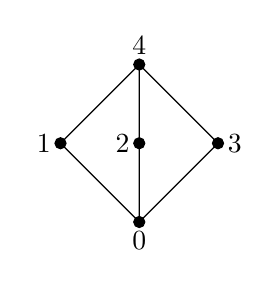
\begin{tikzpicture}
            \filldraw[black] (0,0) circle(2pt) node[above] {4} -- (-1,-1) circle(2pt) node[left] {1} -- (0, -2) circle(2pt) node[below] {0} ;
            \filldraw[black] (0,0) -- (0,-1) circle(2pt) node[left] {2} -- (0, -2) ;
            \filldraw[black] (0,0) -- (1,-1) circle(2pt) node[right] {3} -- (0, -2) ;
        \end{tikzpicture}
        \captionof{figure}{Hasse-Diagramm einer Ordnungsrelation}
    \end{minipage}

    $(\mathcal{P}(M), \cap, \cup, \emptyset, M)$ ist ein beschränkter Verband. $(\mathbb{Q}, \min, \max)$ kann hingegen nicht zu einem beschränkten Verband gemacht werden.
\end{example}

\begin{lemma}
    Jeder Verband $\mathfrak{V} = (V, \wedge, \vee)$ mit endlicher Trägermenge $V = \{v_1, \ldots, v_n\}$ kann zu einem beschränkten Verband gemacht werden.
\end{lemma}
\begin{proof}
    Sei $1 := v_1 \vee \ldots \vee v_n$, dann gilt für beliebiges $j \in \{1, \ldots, n\}$, dass $$v_j \vee 1 = v_j \vee v_1 \vee \ldots \vee v_n =  v_1 \vee \ldots \vee v_j \vee v_j \vee \ldots \vee v_n = v_1 \vee \ldots \vee v_n = 1.$$
    Analoges gilt für $0 := v_1 \wedge \ldots \wedge v_n$. Damit ist $(V, \wedge, \vee, 0, 1)$ ein beschränkter Verband. 
\end{proof}

\begin{definition}
    Eine Algebra $\mathfrak{A} = (A, \wedge, \vee, 0, 1, \,')$ vom Typ $\tau = (2,2,0,0,1)$ heißt \emph{Boole'sche Algebra}\index{Boole'sche Algebra}, wenn
    \begin{itemize}[topsep=0pt, label={--}]
        \item $(A, \wedge, \vee, 0, 1)$ ein beschränkter distributiver Verband ist,
        \item $\forall x \in A: x \wedge x' = 0$ und
        \item $\forall x \in A: x \vee x' = 1$
    \end{itemize}
    gilt.
\end{definition}

\begin{example}
    Für eine Menge $M$ ist $(\mathcal{P}(M), \cap, \cup, \emptyset, M, ')$ mit $'(X) := M \setminus X$ eine Boole'sche Algebra.
\end{example}

\begin{remark}
    Alle Boole'schen Algebren werden durch den Darstellungssatz von Stone bis auf Isomorphie beschrieben.
\end{remark}

\begin{definition}
    Seien $\mathfrak{A} = (A, (f_i^\mathfrak{A})_{i \in I}), \mathfrak{B} = (B, (f_i^\mathfrak{B})_{i \in I})$ zwei Algebren vom selben Typ $\tau = (n_i)_{i \in I}$. Eine Abbildung $\varphi: A \to B$ heißt \emph{Homomorphismus}\index{Homomorphismus}, wenn

    $$\forall i \in I \forall a_1, \ldots, a_{n_i} \in A: \varphi(f_i^\mathfrak{A}(a_1, \ldots, a_{n_i})) = f_i^\mathfrak{B}(\varphi(a_1), \ldots, \varphi(a_{n_i})). $$

    Wir schreiben dann auch $\varphi : \mathfrak{A} \to \mathfrak{B}$.

    Wenn $\varphi$ bijektiv ist, dann heißt die Funktion \emph{Isomorphismus}\index{Isomorphismus}.
    Ist $\mathfrak{A} = \mathfrak{B}$, dann heißt $\varphi$ \emph{Endomorphismus}\index{Endomorphismus}. Ein bijektiver Endomorphismus heißt \emph{Automorphismus}\index{Automorphismus}.
\end{definition}

\begin{definition}
    Zwei Algebren $\mathfrak{A} = (A, (f_i^\mathfrak{A})_{i \in I}), \mathfrak{B} = (B, (f_i^\mathfrak{B})_{i \in I})$ von selben Typ nennen wir \emph{isomorph}\index{isomorph}, wenn es einen Isomorphismus $\varphi: \mathfrak{A} \to \mathfrak{B}$ gibt. Wir schreiben auch $\mathfrak{A} \cong \mathfrak{B}$.
\end{definition}

\begin{example}
    Sei $\mathfrak{A}$ eine Algebra. Wir definieren die Mengen \begin{align*}
        \End(\mathfrak{A}) &:= \{f: A \to A \mid f\text{ ist Endomorphismus}\} \text{ und} \\ \Aut(\mathfrak{A}) &:= \{f: A \to A \mid f\text{ ist Automorphismus}\}.
    \end{align*}

    $(\End(\mathfrak{A}), \circ, \id_A)$ ist dann ein Monoid, das \emph{Endomorphismenmonoid von $\mathfrak{A}$}\index{Endomorphismenmonoid}. Jedes Monoid ist isomorph zu einem Endomorphismenmonoid.
    
    $(\Aut(\mathfrak{A}), \circ, \id_A, {}^{-1})$ ist eine Gruppe, die \emph{Automorphismengruppe von $\mathfrak{A}$}\index{Automorphismengruppe}. Nach dem Satz von Cayley ist jede endliche Gruppe isomorph zu einer Automorphismengruppe.
\end{example}
\section{Körpererweiterungen}

Im Folgenden werden wir oft $K \leq L$ schreiben, dabei ist stets $K$ ein Körper und $L$ ein Oberkörper (beziehungsweise eine Körpererweiterung) davon.

\subsection{Einfache algebraische Erweiterungen}

\begin{definition}
    Sei $K \leq L$, so definieren wir $[L:K]$ als die Dimension von $L$ als Vektorraum über $K$.
\end{definition}

\begin{theorem}[Gradsatz]
    Sei $K \leq E \leq L$, $[L:E],[E:K] < \infty$. Dann ist
    $$ [L:K] = [L:E] \cdot [E:K] < \infty. $$
\end{theorem}

\begin{proof}
    Übungsaufgabe.
\end{proof}

\begin{definition}
    Sei $K \leq L, \alpha \in L$. Dann nennen wir \emph{$\alpha$ algebraisch über $K$}\index{algebraisch} (kurz $\alpha \text{ alg.}/_K$), wenn
    $$ \exists f \in K[x] \setminus \{0\}: f(\alpha) = 0. $$
\end{definition}

\begin{example}
    Sei $K$ ein Körper und betrachte $K \leq K(x)$. Dann ist $x$ nicht algebraisch, da $x$ klarerweise nicht annullierbar ist.
\end{example}

\begin{example}
    Betrachte $\mathbb{R} \leq \mathbb{C}$. Dann ist $i \in \mathbb{C}$ algebraisch$/_\mathbb{R}$, da wir $f(x) = x^2 + 1$ wählen können.
\end{example}

\begin{example}
    Betrachte $\mathbb{Q} \leq \mathbb{R}$. Dann ist $\sqrt{2} \in \mathbb{R}$ algebraisch$/_\mathbb{Q}$. Jedoch sind $\pi, e \in \mathbb{R}$ nicht algebraisch$/_\mathbb{Q}$.
\end{example}

\begin{definition}
    Wir nennen \emph{$\alpha$ transzendent über $K$}\index{transzendent} (kurz $\alpha \text { transz.}/_K$) genau dann, wenn $\alpha$ nicht algebraisch über $K$ ist.
\end{definition}

\begin{remark}
    Ist $\alpha$ algebraisch über $K$, so können wir das nichttriviale Ideal
    $$ I := \{ f \in K[x] \mid f(\alpha) = 0 \} \vartriangleleft K[x] $$
    wählen. Nun gibt es ein $\mu_\alpha \in K[x]$ normiert, mit $I = (\mu_a)$, da $K[x]$ ein Hauptidealring ist. Dieses ist eindeutig bis auf Assoziiertheit, denn ist $I = (\mu_\alpha) = (g)$, so gilt $\mu_\alpha \mid g$ und $g \mid \mu_\alpha$, womit $g \sim \mu_\alpha$. Dieses $\mu_\alpha$ nennen wir das \emph{Minimalpolynom von $\alpha$ über $K$}\index{Minimalpolynom}. Verschiedene $\alpha, \beta$ können dasselbe Minimalpolynom besitzen. In diesem Fall stimmen jedoch die jeweiligen Körpererweiterungen überein, wie wir in folgender Proposition sehen werden.
\end{remark}

\begin{proposition}
    Sei $K \leq L, \alpha \in L$ algebraisch über $K$ und $\deg \mu_\alpha = k$. Dann gilt:
    \begin{enumerate}
        \item Die Abbildung $\varphi : K[x]/_{(\mu_\alpha)} \to K[\alpha], f + (\mu_\alpha) \mapsto f(\alpha)$ ist ein Ring-Isomorphismus.
        \item $K[\alpha] = K(\alpha)$
        \item $\forall \beta \in K(\alpha) \exists ! a_0, \hdots, a_{k-1} \in K: \beta = \sum_{i=0}^{k-1}a_i \alpha^i$
        \item $\alpha^0, \hdots, \alpha^{k-1}$ bildet eine Basis von $K(\alpha)/_K$ als Vektorraum.
        \item $[K(\alpha) : K] = k$
        \item Ist $\beta \in L, \mu_\alpha = \mu_\beta$, so existiert ein eindeutiger Isomorphismus $\psi : K(\alpha) \to K(\beta)$ mit $\psi(\alpha) = \beta$ und $\psi\vert_K = \id_K$.
    \end{enumerate}
\end{proposition}

\begin{proof}{\ }
    \begin{enumerate}
        \item Folgt sofort aus dem Homomorphiesatz, angewandt auf den Einsetzungshomomorphismus.
        
        \item Es ist $K[\alpha]$ ein Unterring von $L$ und damit ein Integritätsbereich. Nach (1) ist also auch $K[x]/_{(\mu_\alpha)}$ ein Integritätsbereich, womit $(\mu_\alpha)$ prim ist. Damit ist $\mu_\alpha$ prim, insbesondere irreduzibel. Wir behaupten nun, dass $(\mu_\alpha)$ ein maximales Ideal ist. Um dies einzusehen sei $J$ ein echtes Ideal von $K[x]$ mit $(\mu_\alpha) \subseteq J$. Dann gibt es ein $g \in K[x]$ mit $J = (g)$, also $(\mu_\alpha) \subseteq (g)$, womit $g \mid \mu_\alpha$ folgt. Da $\mu_\alpha$ irreduzibel ist folgt dadurch $g \sim \mu_\alpha$ und damit $J = (\mu_\alpha)$. Also ist $(\mu_\alpha)$ maximal. Damit ist jedoch $K[x]/_{(\mu_\alpha)}$ ein Körper und nach (1) isomorph zu $K[\alpha]$, womit $K[\alpha] = K(\alpha)$ folgt.
        
        \item Existenz: Nach (1) und (2) gibt es ein $f \in K[x]$ mit $\varphi(f + (\mu_\alpha)) = f(\alpha) = \beta$. Nun ist $f = g \cdot \mu_\alpha + f'$ mit einem Polynom $f'$ mit Grad kleiner $k$. Damit ist $f'(\alpha) = f(\alpha) = \beta$.
        
        Eindeutigkeit: Ist $f(\alpha) = \beta = g(\alpha)$, wobei der Grad von $f, g$ kleiner als $k$ ist, so folgt $(f-g)(\alpha) = 0$, womit $(f-g) \in (\mu_\alpha)$ liegt, also gilt $\mu_\alpha \mid (f-g)$, womit $f-g=0$ und damit $f=g$ ist.

        \item Folgt sofort aus (3).
        
        \item Folgt sofort aus (4).
        
        \item {Existenz:} Nach (1) gibt und (2) gibt es Isomorphismen
        $\varphi:K[x]/_{(\mu_\alpha)}\to K(\alpha)$ und $\varphi':K[x]/_{(\mu_\alpha)}\to K(\beta)$
        welche $\varphi\vert_K=\id_K$ und $\varphi'\vert_K=\id_K$ erfüllen. Wegen $\varphi(x+(\mu_\alpha))=\alpha$
        und $\varphi'(x+(\mu_\alpha))=\beta$ liefert $\varphi'\circ\varphi^{-1}:K(\alpha)\to K(\beta)$
        einen gewünschten Isomorphismus.

        {Eindeutigkeit:} Sei $\psi:K(\alpha)\to K(\beta)$ ein Isomorphismus mit $\psi(\alpha)=\beta$
        und $\psi\vert_K=\id_K$. Dann gilt insbesondere $\psi(\alpha^i)=\beta^i$, da $\psi$ ein Körperautomorphismus
        ist. Daher ist $\psi$ als lineare Abbildung von $K(\alpha)$ als Vektorraum über $K$ in den Vektorraum $K(\beta)$
        bereits auf einer Basis eindeutig festgelegt, womit $\psi$ istbesondere als Körperautomorphismus eindeutig ist.
    \end{enumerate}
\end{proof}

\subsection{Nicht-einfache algebraische Erweiterungen}

\begin{definition}
    Wir nennen $K \leq L$ \emph{(rein) algebraisch}\index{Körpererweiterung!rein algebraisch}\index{algebraisch}, wenn
    $$ \forall \alpha \in L: \alpha \text{ ist algebraisch über } K. $$
\end{definition}

\begin{proposition}{\ }
    \begin{enumerate}
        \item Sei $K \leq L$. Gilt $[L:K] < \infty$, so ist $K \leq L$ algebraisch.
        \item Sei $K \leq K(\alpha)$ algebraisch, so ist $[K(\alpha) : K] < \infty$.
        \item Sei $K \leq L$ algebraisch und $L \leq M$ algebraisch, so ist $K \leq M$ algebraisch.
        \item Sei $K \leq L$ und $S := \{ \alpha \in L \mid \alpha \text{ ist algebraisch über } K \}$, so ist $K \leq S \leq L$.
    \end{enumerate}
\end{proposition}

\begin{proof}{\ }
    \begin{enumerate}
        \item Sei $\alpha \in L \setminus \{0\}$. Da die Dimension der Erweiterung endlich ist, ist die Folge der Potenzen $\alpha^0, \alpha^1, \hdots$ linear abhängig über K. Es gibt also $a_0, \hdots, a_n \in K$ mit $\sum_{i=0}^n a_i \alpha^i = 0$, womit wir $f(x) = \sum_{i=0}^n a_i x^i$ wählen können. Es ist $f(\alpha) = 0$, womit $\alpha$ algebraisch ist.
        
        \item Es gilt $[K(\alpha) : K] = \deg \mu_\alpha < \infty$.
        
        \item Sei $\alpha \in M$ beliebig, so gibt es ein $f(x) = \sum_{i=0}^n a_i x^i \in L[x], f(\alpha) = 0$, wobei $a_i \in L$, also algebraisch über $K$ sind. Es ist dann auch $\alpha$ algebraisch über $K(a_0, \hdots, a_n)$. Nun gilt
        \begin{align*}
            [K(\alpha) : K] &\leq [K(\alpha, a_0, \hdots, a_n) : K] = \\
            &= [K(\alpha, a_0, \hdots, a_n) : K(a_0, \hdots, a_n)] \cdot [K(a_0, \hdots, a_n) : K] = \\
            &= [K(\alpha, a_0, \hdots, a_n) : K(a_0, \hdots, a_n)] \cdot \hdots \cdot [K(a_n) : K] < \infty
        \end{align*}
        und nach (1) ist $K$ algebraisch.

        \item Seien $\alpha, \beta \in S$. Dann gilt auch $\alpha, \beta \in K(\alpha, \beta) \subseteq S$. Nach (1) ist $K \leq K(\alpha)$ algebraisch, genauso ist $K(\alpha) \leq K(\alpha, \beta)$ algebraisch, wobei letzteres ein Körper ist, womit $\alpha \cdot \beta, \alpha + \beta, \alpha^{-1} \in K(\alpha, \beta)$ folgt und wir damit nach (3) algebraisch über K sind.
    \end{enumerate}
\end{proof}

\subsection{Transzendente Erweiterungen}

\begin{proposition}
    Sei $K \leq L, \alpha \in L$ transzendent über $K$. Dann existiert ein eindeutiger Isomorphismus $\psi : K(x) \to K(\alpha)$ mit $\psi(x) = \alpha, \psi \vert_K = \id_K$.
\end{proposition}

\begin{proof}
    Existenz: Sei $\varphi : K[x] \to K[\alpha]$ der Einsetzungshomomorphismus, $\varphi(f(x)) = f(\alpha)$. Da $\alpha$ transzendent ist, ist $\ker \varphi$ trivial. Damit ist $\varphi$ ein Ringisomorphismus. Nun ist $K(x)$ der Quotientenkörper von $K[x]$, genauso ist $K(\alpha)$ der Quotientenkörper von $K[\alpha]$. Aufgrund der Eindeutigkeit des Quotientenkörpers existiert genau ein $\psi : K(x) \to K(\alpha)$ mit $\psi\vert_{K[x]} = \varphi$.

    Eindeutigkeit: Sei $\widetilde{\psi}$ ein weiterer Isomorphismus mit denselben Eigenschaften. Damit folgt $\widetilde{\psi}\vert_{K[x]} = \varphi$. Nach der oben erwähnten Eindeutigkeit des Quotientenkörpers folgt dadurch bereits $\widetilde{\psi} = \psi$.
\end{proof}

\notedate{31.05.2023}

\begin{definition}
    Sei $K \leq E$.
    \begin{itemize}
        \item Sei $S \subseteq E$. Wir nennen $S$ \emph{algebraisch abhängig über $K$}\index{algebraisch abhängig}, wenn es $a_1,\hdots,a_n\in S$ paarweise verschieden und $ f(x_1, \hdots, x_n) \in K[x_1, \hdots, x_n], f \neq 0$ mit $f(a_1,\hdots,a_n)=0$ gibt.
        Sonst nennen wir $S$ \emph{algebraisch unabhängig}\index{algebraisch unabhängig}.
        \item Wir $E$ \emph{rein transzendent über $K$}\index{transzendent!rein}, wenn es eine algebraisch unabhängige Teilmenge $S \subseteq E$ gibt mit $E = K(S)$.
        \item Sei $S \subseteq E$. Wir nennen $S$ \emph{Transzendenzbasis von $E$ über $K$}\index{Transzendenzbasis}, wenn $S$ maximal algebraisch unabhängig ist.
    \end{itemize}
\end{definition}

\begin{remark}
    Sei $S$ eine Transzendenzbasis von $E$ über $K$, so bedeutet das \emph{nicht} $E = K(S)$, wie wir gleich sehen werden.
\end{remark}

\begin{proposition}
    Sei $K \leq E, S \subseteq E$. Dann sind äquivalent:
    \begin{enumerate}
        \item $S$ ist maximal algebraisch unabhängig, also eine Transzendenzbasis.
        \item $S$ ist minimal, sodass $E$ algebraisch über $K(S)$ ist.
        \item $S$ ist algebraisch unabhängig und $E$ ist algebraisch über $K(S)$.
    \end{enumerate}
\end{proposition}

\begin{proof}
    Übungsaufgabe.
\end{proof}

\begin{proposition}
    Seien $K \leq L_1, L_2$ und $S_1 \subseteq L_1, S_2 \subseteq L_2$ algebraisch unabhängig über $K$, sowie $\varphi : S_1 \to S_2$ eine Bijektion. Dann gibt es eine eindeutige Fortsetzung $\overline{\varphi} : K(S_1) \to K(S_2)$ sodass $\overline{\varphi}$ ein Isomorphismus ist und $\overline{\varphi} \vert_K = \id_K, \overline{\varphi} \vert_{S_1} = \varphi$.
\end{proposition}

\begin{proof}
    Übungsaufgabe.
\end{proof}

\begin{proposition}
    Sei $K \leq E$, dann gibt es eine Transzendenzbasis $S$ von $E$ über $K$.
\end{proposition}

\begin{proof}
    Betrachte
    $$ S := \{ S \subseteq E \mid S \text{ ist algebraisch unabhängig über } K \}. $$
    Ist $S = \emptyset$ so ist $\emptyset$ bereits eine Transzendenzbasis. Sonst ist $(S, \subseteq)$ eine Halbordnung und ist $K \subseteq S$ eine Kette, so ist $\bigcup K \in S$. Nach dem Lemma von Zorn gibt es ein maximales Element, welches gerade unsere Transzendenzbasis darstellt.
\end{proof}

\begin{corollary}
    Sei $K \leq E$ und $S \subseteq E$ eine Transzendenzbasis von $E$ über $K$. Dann ist $K \leq K(S) \leq E$, wobei der erste Schritt (von $K$ auf $K(S)$) rein transzendent und der zweite Schritt (von $K(S)$ auf $E$) rein algebraisch ist.
\end{corollary}

\begin{definition}
    Sei $K \leq E, A \subseteq E$. Dann definieren wir die \emph{algebraische Hülle von $A$}\index{algebraische Hülle} als
    $$ [A] := \{ b \in E \mid b \text{ ist algebraisch über } K(A) \}. $$
    Gilt $E = [A]$, so heißt $A$ \emph{algebraisches Erzeugendensystem von $E$ über $K$}\index{algebraisches Erzeugendensystem}.
\end{definition}

\begin{lemma}
    Sei $K \leq E, A \subseteq E$. Dann gilt $[[A]] = [A]$.
\end{lemma}

\begin{proof}
    Es gilt $K(A) \leq [A]$ als Körper, sowie $[A] \leq [[A]]$. Beide dieser Körpererweiterungen sind algebraisch, womit auch $K(A) \leq [[A]]$ eine algebraische Erweiterung ist. Also gilt für alle $b \in [[A]]$ bereits $b \in [A]$.
\end{proof}

\begin{lemma}[Austauschlemma]
    Seien $K \leq E, A \subseteq E, b, c \in E$ mit $c \in [A \cup \{b\}], c \notin [A]$. Dann ist $b \in [A \cup \{c\}]$.
\end{lemma}

\begin{proof}
    Sei $f \in K(A \cup \{b\})[x] \setminus \{0\}$ das entsprechende Polynom bezüglich $c$, \obda gelte $f \in K[A \cup \{b\}][x]$. Sei $g(x,y) \in K[A][x,y]$ mit $g(x,b) = f(x)$. Wähle $h(y) := g(c, y) \in K[A \cup \{c\}][y]$. Dann ist $\deg h(y) \geq 1$. Nun gilt $h(b) = g(c,b) = f(c) = 0$, womit $b$ algebraisch über $K(A \cup \{ c \})$ ist.
\end{proof}

\begin{corollary}
    Seien $K \leq E, A \subseteq E, b, c \in E$ mit $c \in [A \cup \{b\}], c \notin [A]$. Dann gilt:
    \begin{itemize}
        \item $[A \cup \{b\}] = [A \cup \{c\}]$
        \item Ist $A$ algebraisch unabhängig, so ist auch $A \cup \{ b \}$ algebraisch unabhängig.
    \end{itemize}
\end{corollary}

\begin{proof}
    Es ist $c \in [A \cup \{b\}]$, womit $[A \cup \{c\}] \subseteq [A \cup \{b\}]$ folgt. Mit dem Austauschlemma folgt die andere Mengeninklusion.

    Sei nun $A$ algebraisch unabhängig. Wäre $A \cup \{ b \}$ algebraisch abhängig, so wäre $b \in [A]$ und damit $c \in [A]$, im Widerspruch.
\end{proof}

\begin{corollary}
    Seien $B, C$ Transzendenzbasen von $E$ über $K$. Dann gibt es für alle $b \in B$ ein $c \in C$, sodass $(B \setminus \{b\}) \cup \{c\}$ eine Transzendenzbasis ist.
\end{corollary}

\begin{proof}
    Zunächst gibt es ein $c \in C$ mit $c \notin [B \setminus \{b\}]$, da wir sonst eine kleinere Transzendenzbasis hätten. Wegen $c \in [B]$ folgt mit dem Austauschlemma, dass $b \in [(B \setminus \{b\}) \cup \{c\}]$. Damit ist $E$ algebraisch über $[(B \setminus \{b\}) \cup \{c\}]$. Weiters ist $[(B \setminus \{b\}) \cup \{c\}]$ algebraisch unabhängig.
\end{proof}

\begin{lemma}
    Seien $K \leq E$, $B, C$ Transzendenzbasen und $B$ endlich. Dann ist $\vert B \vert = \vert C \vert$.
\end{lemma}

\begin{proof}
    Wir tauschen induktiv Basisvektoren aus. Dazu sei $B_0:=B=\{b_1,\ldots,b_n\}$. Wähle $c_0 \in C_0$, sodass $B_{1}:=B\setminus\{b_0\}\cup\{c_0\}$ eine Transzendenzbasis ist. Es ist $c_0\not\in B\setminus\{b_0\}$, da sonst $B$ keine Transzendenzbasis wäre. Fährt man induktiv fort, so erhält man nach $n$-Schritten, dass $B_n\subseteq C$ eine Transzendenzbasis ist, also folgt
    $|B|=|B_n|=|C|$.
\end{proof}

\begin{theorem}
    Seien $K \leq E$, $B, C$ Transzendenzbasen. Dann ist $\vert B \vert = \vert C \vert$.
\end{theorem}

\begin{proof}
    Sind $B$ oder $C$ endlich so folgt die Aussage aus dem vorigen Lemma. Seien also $B,C$ unendlich. Es gibt für alle $c \in C$ ein $B_c \subseteq B$ endlich mit $c \in [B_c]$. Es gilt $\bigcup_{c \in C} B_c = B$, womit $\vert B \vert \leq \sum_{c \in C} \vert B_c \vert = \vert C \vert$ folgt. Aus Symmetriegründen folgt die andere Ungleichung und damit die Gleichheit.
\end{proof}

\begin{definition}
    Sei $K \leq E$. Wir definieren den \emph{Transzendenzgrad von $E$ über $K$}\index{Transzendenzgrad} als $\vert B \vert$, wobei $B \subseteq E$ eine beliebige Transzendenzbasis ist.
\end{definition}

\subsection{Adjunktion einer Nullstelle}

\begin{lemma}
    Sei $K$ ein Körper, $f \in K[x]$ irreduzibel mit $\deg f \geq 2$. Dann hat $f$ keine Nullstellen in $K$.
\end{lemma}

\begin{proof}
    Wir behaupten $f(a) = 0 \Leftrightarrow (x-a) \mid f$. Die Implikation von rechts nach links ist klar. Ist $a$ eine Nullstelle von $f$, so können wir mit dem Divisionsalgorithmus $f(x) = q \cdot (x-a) + r(x)$ mit $\deg r < 1$ schreiben. Dann ist $0 = f(a) = 0 + r(0)$, womit $r = 0$ folgt und die Aussage gezeigt ist.
\end{proof}

\begin{example}
    Betrachte $\mathbb{R} \leq \mathbb{C}$. Es ist $f(x) = x^2 + 1$ irreduzibel über $\mathbb{R}$. Wir wollen $i$ zu einer Nullstelle machen, dann gilt also $i^2 + 1 = 0$. Damit können wir auf $i^3 = i \cdot i^2 = i \cdot (-1)$ schließen, analog für $i^4, \hdots$. Wir können also das Verhalten von $i$ nur durch die Eigenschaft eine Nullstelle zu seien analysieren.
\end{example}

\begin{proposition}[Kronecker]
    Sei $f \in K[x]$ irreduzibel. Dann gilt:
    \begin{enumerate}
        \item $K[x] /_{(f)} =: L$ ist ein Körper.
        \item Die Abbildung $\varphi : K \to L, c \mapsto c + (f)$ ist eine Körpereinbettung.
        \item Es gibt eine eindeutige Ringbettung $\overline{\varphi} : K[x] \to L[x]$ mit $\overline{\varphi} \vert_K = \varphi, \overline{\varphi}(x) = x$.
        \item Identifiziert man $K[x]$ mit $\varphi(K[x])$ und $K$ mit $\varphi(K)$, so ist
        $x + (f) \in L$  eine Nullstelle von $f$ (formal von $\overline{\varphi}(f)$).
        \item $[L : K] = \deg f < \infty$, insbesondere ist $L$ algebraisch über $K$.
    \end{enumerate}
\end{proposition}
\notedate{01.06.2023}
 
\begin{proof}{\ }
    \begin{enumerate}
        \item Es ist nur zu zeigen, dass $f$ ein maximales Ideal ist, da dann bereits die Aussage aus \cref*{prop:ringideale} folgt. In Hauptidealringen sind die maximalen Ideale gerade die von den irreduziblen Elementen erzeugten Ideale -- da $K[x]$ ein Hauptidealring ist, folgt also das zu Zeigende.
        \item Klarerweise ist $\varphi$ ein Homomorphismus. Für die Injektivität betrachten wir $c + (f) = d + (f)$. Es ist also $c - d \in (f)$, also $f \mid c - d$, womit jedoch bereits $c = d$ folgt.
        \item Klarerweise ist $\overline{\varphi}$ ein Homomorphismus. Für die Injektivität betrachten wir $\overline{\varphi}(g) = \overline{\varphi}(h)$, wegen Koeffizientenvergleich müssen dann jedoch bereits die Polynome übereinstimmen, es gilt also $g = h$. Für die Eindeutigkeit bemerken wir, dass $K[x]$ von $K \cup \{ x \}$ erzeugt wird. Quasi ist $K[x]$ also frei erzeugt von $x$ über $K$.
        \item Es ist $f(x + (f)) = f(x) + (f) = 0 + (f) = 0_L$, da $f(x) \in (f)$.
        \item Es gilt $L = K(x + (f))$, da $K[x]$ von $K \cup \{x\}$ erzeugt wird. Weiters ist gerade $f$ das Minimalpolynom von $x + (f)$ über $K$, womit $[L : K] = \deg f$ folgt.
    \end{enumerate}
\end{proof}

\begin{definition}
    Sei $K \leq E$ und $P \subseteq K[x]$.
    \begin{itemize}
        \item $E$ heißt \emph{Nullstellenkörper} von $P$ (über $K$), wenn jedes $f \in P$ über $E$ in Linearfaktoren zerfällt, das heißt es gibt $\alpha_1, \hdots, \alpha_n \in E, a \in K$ mit $f(x) = a(x - \alpha_1) \hdots (x - \alpha_n)$, wobei die Linearfaktoren nicht paarweise verschieden sein müssen.
        \item Wenn $E$ minimal mit dieser Eigenschaft ist (das heißt, dass $E$ von $K$ und den Nullstellen von $f \in P$ erzeugt wird), dann heißt $E$ \emph{Zerfällungskörper} von $P$ (über $K$).
        \item $K$ heißt \emph{algebraisch abgeschlossen}, wenn jedes nichtkonstante Polynom in $K[x]$ über $K$ in Linearfaktoren zerfällt.
        \item Ein \emph{algebraischer Abschluss} von $K$ ist ein Erweiterungskörper $L$, sodass $K \leq L$ algebraisch und $L$ algebraisch abgeschlossen ist.
    \end{itemize}
\end{definition}

\begin{example}
    Betrachte $K = \mathbb{Q}, P = \{ x^2 - 2 \}$, so ist $E = \mathbb{Q}(\sqrt{2})$ ein Zerfällungskörper.
    
    Mit $P = \{ x^3 - 2 \}$ ist beispielsweise $\mathbb{C}$ ein Nullstellenkörper. Es ist $\mathbb{Q}(\sqrt[3]{2})$ \emph{kein} Zerfällungskörper und auch kein Nullstellenkörper, da die komplexen Wurzeln fehlen. $\mathbb{Q}(\sqrt[3]{2}, \sqrt[3]{2} e^{\frac{2 \pi i}{3}}, \sqrt[3]{2} e^{\frac{4 \pi i}{3}})$ hingegen ist ein Zerfällungskörper.
\end{example}

\begin{remark}
    Wie wir später sehen werden sind Zerfällungskörper (bis auf Isomorphie) eindeutig -- es macht also durchaus Sinn von \emph{dem} Zerfällungskörper zu sprechen.
\end{remark}

\begin{proposition}
    Sei $K$ ein Körper, dann sind äquivalent:
    \begin{enumerate}
        \item $K$ ist algebraisch abgeschlossen.
        \item Jedes nicht konstante Polynom in $K[x]$ hat eine Nullstelle in $K$.
        \item Jedes nicht konstante irreduzible Polynom in $K[x]$ hat eine Nullstelle in $K$.
        \item Jedes nicht konstante irreduzible Polynom in $K[x]$ hat Grad 1.
        \item Für jede algebraische Erweiterung $L \geq K$ gilt $L = K$.
    \end{enumerate}
\end{proposition}

\begin{proof}
    Übungsaufgabe.
\end{proof}

\begin{proposition}
    Sei $K \leq L$, dann sind äquivalent:
    \begin{enumerate}
        \item $L$ ist ein algebraischer Abschluss von $K$.
        \item $L$ ist ein Nullstellenkörper von $K[x]$ und $L$ ist algebraisch über $K$.
        \item $L$ ist ein Zerfällungskörper von $K[x]$.
        \item $L$ ist algebraisch über $K$ und für alle $L' \geq L$ gilt, dass wenn $L'$ algebraisch über $K$ ist, dann ist bereits $L' = L$.
    \end{enumerate}
\end{proposition}

\begin{proof}
    Übungsaufgabe.
\end{proof}

\begin{proposition}\label{prop:alg_abschluss}
    Sei $K$ ein Körper. Dann gibt es einen Zerfällungskörper von $K[x]$ über $K$. Dieser ist insbesondere algebraisch. Damit gibt es insbesondere einen algebraischen Abschluss von $K$.
\end{proposition}

\begin{proof}
    Wir geben einen Beweis an, welcher die Idee besonders gut widerspriegelt, allerdings technisch nicht korrekt ist, siehe dazu auch die nächste Bemerkung. Betrachte
    $$ \mathcal{S} := \{ E \mid E \text{ ist Körper}, K \leq E \text{ algebraische Erweiterung } \}. $$
    Dann ist $(\mathcal{S}, \leq)$ eine Halbordnung. Klarerweise ist $\mathcal{S} \neq \emptyset$, da zumindest $K\in \mathcal{S}$ gilt, weiters sind alle Ketten beschränkt. Um dies einzusehen, sei $\mathcal{K} = \{ E_i \mid i \in I \}$ eine Kette in $\mathcal{S}$. Wir wollen ein $E \in \mathcal{S}$ finden mit $E_i \leq E$ für alle $i \in I$. Wähle dazu $E := \bigcup_{i \in I} E_i$. Wie man (aufgrund der Ketteneigenschaft) verifiziert, ist $E$ ein Oberkörper, wobei $x+y:=x+^{E_i}y$ mit einem $i\in I$ sodass $x,y\in E_i$ gilt definiert wird. Aufgrund der Ketteneigenschaft ist die Definition unabhängig von der Wahl von $i$, das heißt die Addition auf $E$ ist wohldefiniert, die anderen Operationen definiert man analog. Klarerweise gilt auch $K \leq E$. Da alle Elemente der Vereinigung algebraisch sind, ist auch $E$ algebraisch, womit tatsächlich $E \in \mathcal{S}$ folgt. Mit dem Lemma von Zorn erhalten wir also ein maximales $E \in \mathcal{S}$. Wir wollen zeigen, dass $E$ algebraisch abgeschlossen ist, da dann $E$ bereits der Zerfällungskörper ist. Sei dazu $f \in E[x]$ irreduzibel, wir wollen zeigen, dass $f$ eine Nullstelle in $E$ hat. Nach Kronecker gibt es ein $E_1 \in \mathcal{S}$ sodass $E \leq E_1$ eine algebraische Erweiterung ist und $f$ eine Nullstelle in $E_1$ hat. Da $E$ maximal ist folgt jedoch $E_1 = E$, womit das zu Zeigende folgt.
\end{proof}

\begin{remark}
    Streng genommen ist der obige Beweis ``falsch'', da $\mathcal{S}$ keine Menge sein muss. Da es beliebig viele isomorphe algebraische Körpererweiterungen gibt (mittels Umbenennung) ist $\mathcal{S}$ im Allgemeinen eine echte Klasse, womit wir das Lemma von Zorn nicht mehr anwenden können.

    Wir reparieren dies, indem wir stattdessen definieren
    $$ \mathcal{S} = \{ E \mid E \text{ ist Körper}, K \leq E \text{ algebraische Erweiterung}, E \subseteq X \} $$
    mit einer festen Menge $X$. Dann ist nämlich
    $$ \mathcal{S} \subseteq \mathcal{P}(X) \times \mathcal{P}((X \times X) \times X) \times \hdots, $$
    wobei die Potenzmengen gerade die Körperoperationen umfangen, und damit eine Menge.

    Bleibt zu klären was $X$ sein soll. Wir wählen $X$ als eine beliebige Menge mit $\vert X \vert > \max(\vert K \vert, \vert \mathbb{N} \vert)$. Beispielsweise könnte man $X = K \cup \mathcal{P}(K) \cup \mathbb{R}$ wählen.

    Weiters muss man noch darauf achten, dass $E_1$ hier nicht unbedingt in $\mathcal{S}$ sein muss. Da $E_1$ jedoch vergleichsweise ``klein'' ist können wir $E_1$ problemlos in eine Menge $\widetilde{E_1} \in \mathcal{S}$ umbenennen.
\end{remark}

\begin{proposition}
    Sei $K \leq L$ algebraisch. Dann gilt $\vert L \vert \leq \max(\vert K \vert, \vert \mathbb{N} \vert)$.
\end{proposition}

\begin{proof}
    Sei $a \in L$, dann gibt es ein $f \in K[x] \setminus \{0\}$ mit $f(\alpha) = 0$. Nun ist
    $$ N_f := \{ \beta \in L \mid f(\beta) = 0 \} $$
    endlich. Weiters ist
    $$ L \subseteq \bigcup_{f \in K[x] \setminus \{0\}} N_f, $$
    womit wegen $\vert K[x] \vert = \max(\vert K \vert, \vert \mathbb{N} \vert)$ folgt $\vert L \vert \leq \vert K[x] \vert \cdot \vert \mathbb{N} \vert = \max(\vert K \vert, \vert \mathbb{N} \vert)$.
\end{proof}

\notedate{07.06.2023}

\begin{theorem}\label{theorem:zerfaellungskoerper_existenz}
    Sei $K$ ein Köper, dann gilt:
    \begin{enumerate}
        \item $\forall P \subseteq K[x] \exists Z_P \ge K \;\text{Zerfällungskörper}\;\land Z_P \;\text{alg.}/_K$
        \item $Z := Z_{K[x]}$ ist algebraisch abgeschlossen.
    \end{enumerate}
\end{theorem}
\begin{proof}
    Die zweite Behauptung wird in \cref{prop:alg_abschluss} gezeigt. Zeigen wir also noch die erste Aussage. Sei $P \subseteq K[x]$ beliebig und definieren wir $Z_P := K(S)$ mit $S := \{\alpha \in Z_{K[x]} \mid \exists f \in P\setminus\{0\}: f(\alpha) = 0 \}$. $Z_P$ ist ein Nullstellenkörper von P, da er um genau um die Nullstellen erweitert wird. Die Minimalität von $Z_P$ folgt aus der Konstruktion.
\end{proof}

\begin{theorem}\label{theorem:zerfaellungskoerper_isomorph}
    Seien $K$ ein Körper, $P \subseteq K[x]$ und $Z_1, Z_2$ Zerfällungskörper von $P$ über $K$. Es gibt dann einen Isomorphismus $\varphi: Z_1 \to Z_2$ mit $\varphi\vert_K = \id_K$. 
\end{theorem}

\begin{remark}
    Im Allgemeinen ist der Isomorphismus aus \cref{theorem:zerfaellungskoerper_isomorph} nicht eindeutig.

    Betrachten wir zum Beispiel $\mathbb{R} \le \mathbb{C}$ und $\varphi: \mathbb{C} \to \mathbb{C}, z \to \overline{z}$, so ist $\varphi$ ein Automorphismus mit $\varphi\vert_\mathbb{R} = \id_\mathbb{R}$. Die Identität ist allerdings ein zweiter Isomorphismus der $\mathbb{R}$ festhält.

    Es ist für einen Körper $K$ und einen algebraischen Abschluss $\overline{K}$ die Menge $\Aut_K(\overline{K})\footnote{Diese Gruppe wird auch als Galoisgruppe bezeichnet} = \{ \varphi \in \Aut(\overline{K}) \mid \varphi\vert_K = \id_K \}$  mit der Komposition eine Gruppe. Die Galoistheorie stellt einen Zusammenhang zwischen dieser Gruppe und den Körpererweiterungen her.
\end{remark}

\begin{proof}[Beweis von \cref{theorem:zerfaellungskoerper_isomorph}]
    Betrachten wir $$\mathcal{S} := \{\widetilde{\varphi} \mid L\le \dom \widetilde\varphi \le Z_1, K\le \ran \widetilde\varphi \le Z_2, \widetilde\varphi\;\text{Isomorphismus}\;, \widetilde\varphi\vert_K = \id_K \},$$
    so stellen wir fest, dass $(\mathcal{S}, \subseteq)$ eine Halbordnung ist, $\mathcal{S} \neq \emptyset$, da $\id_K \in \mathcal{S}$ und für jede Kette $K \subset \mathcal{S}$ auch $\bigcup K \in \mathcal{S}$ ist. Nach dem Lemma von Zorn folgt die Existenz eines maximalen Elements $\varphi$ in $\mathcal{S}$.

    Wir zeigen, dass für $\widetilde\varphi \in \mathcal{S}$ mit $\dom \widetilde\varphi \neq Z_1$ ein $\widehat\varphi \in \mathcal{S}$ existiert mit $\widehat\varphi \supsetneq \widetilde\varphi$.
    
    Es ist $Z_1$ ein minimaler Nullstellenkörper von $P$, also existieren $f \in P$ und $\alpha \in Z_1\setminus\dom \widetilde{\varphi}$ mit $f(\alpha) = 0$. Sei $\mu_\alpha$ das Minimalpolynom von $\alpha$ über $\dom \widetilde\varphi$, also $\mu_\alpha \in (\dom \widetilde\varphi)[x]$. Als Minimalpolynom ist $\mu_\alpha$ irreduzibel über $\dom \widetilde\varphi$. Wenden wir nun $\widetilde\varphi$ auf die Koeffizienten von $\mu_\alpha$ an und schreiben dafür $\widetilde\varphi(\mu_\alpha)$, dann ist auch $\widetilde\varphi(\mu_\alpha)$ irreduzibel in $\ran \widetilde\varphi$ und aus $\mu_\alpha \mid f$ folgt $\widetilde\varphi(\mu_\alpha) \mid f$. 
    Es zerfällt $f$ über $Z_2$ in Linearfaktoren (da $f \in P$) und wegen $\widetilde\varphi(\mu_\alpha) \mid f$ zerfällt damit auch $\widetilde\varphi(\mu_\alpha)$ über $Z_2$ in Linearfaktoren. Es gibt daher ein $\beta \in Z_2$ mit $\widetilde\varphi(\mu_\alpha)(\beta) = 0$. Da $\widetilde\varphi(\mu_\alpha)$ als Minimalpolynom irreduzibel über $\ran \widetilde\varphi$ ist, erhält man $\beta \not\in \ran \widetilde\varphi$.  $\widetilde\varphi(\mu_\alpha)$ ist also das Minimalpolynom von $\beta$, womit es ein $\widehat\varphi: (\dom \widetilde\varphi)(\alpha) \to (\ran \widetilde\varphi)(\beta)$ mit $\widehat\varphi\vert_{\dom \widetilde\varphi} = \widetilde\varphi$ und $\widehat\varphi(\alpha) = \beta$ gibt.

    Es muss nun also $\varphi$ auf ganz $Z_1$ definiert sein, da wir es sonst wie eben gezeigt erweitern könnten, was ein Widerspruch zur Maximalität wäre. Dass $\ran \varphi = Z_2$ ist erhält man entweder indem man den Beweis mit vertauschten Rollen wiederholt oder mit folgendem Widerspruch. Sei indirekt angenommen $\ran \varphi \subsetneq Z_2$. Es ist $\ran \varphi$ ein Nullstellenkörper, da er isomorph zu $Z_1$ ist. Dies ist ein Widerspruch zur Minimalität von $Z_2$ als Zerfällungskörper.
\end{proof}

\begin{corollary}
    Sei $K$ ein Körper, $Z \ge K$ Zerfällungskörper von $P \subseteq K[x]$, dann ist $Z$ algebraisch über $K$.
\end{corollary}
\begin{proof}
    Wir kennen einen algebraischen Zerfällungskörper und da alle anderen isomorph zu diesem sind, sind alle algebraisch.
\end{proof}

\begin{remark}
    Die \cref{theorem:zerfaellungskoerper_existenz,theorem:zerfaellungskoerper_isomorph} liefern die Existenz und Eindeutigkeit bis auf Isomorphie von algebraischen Abschlüssen. Damit ist die folgende Definition sinnvoll.
\end{remark}

\begin{definition}
    Sei $K$ ein Körper, dann schreiben wir $\overline{K}$ für den algebraischen Abschluss.
\end{definition}

\begin{remark}
    Es gilt $\mathbb{Q} \le \overline{\mathbb{Q}} \le \mathbb{C}$. Die erste Erweiterung ist eine algebraische, abzählbare Erweiterung von $\mathbb{Q}$. Die zweite Erweiterung ist transzendent und überabzählbar.
\end{remark}

\subsection{Mehrfache Nullstellen}
Es stellt sich die Frage, wann ein irreduzibles $f \in K[x]$ in $\overline{K}$ mehrfache Nullstellen hat.

\begin{definition}
    Sei $p \in K[x]$ mit einer Darstellung
    $$ p(x) = q(x) \cdot \prod_{i=1}^n (x-\alpha_i)^{e_i} $$
    mit paarweise verschiedenen $\alpha_i$, $e_i \in \mathbb{N}^+$ und $q \in K[x]$ ohne Nullstellen. Wir nennen $e_i$ die \emph{Vielfachheit}\index{Vielfachheit} der Nullstelle $\alpha_i$. Ist $e_i > 1$, so nennen wir $\alpha_i$ \emph{mehrfache Nullstelle}\index{mehrfache Nullstelle}.
\end{definition}

% TODO:
\begin{example}
    Sei $f(x) = x^p - 1$ mit $p \in \mathbb{P}$.

    Betrachten wir $K = \mathbb{Q}$: $e^\frac{2 \pi i k}{p}$ mit $k = 0, \ldots p-1$ sind verschiedene (einfache) Nullstellen und bereits alle.

    Betrachten wir $K$ mit $\chara K = p$. Es ist $x^p - 1 = x^p - 1^p = (x-1)^p$. Es gibt also nur die $p$-fache Nullstelle $1$.
\end{example}

\begin{definition}
    Sei $K$ ein Körper, $f(x) = \sum_{i=0}^n a_i x^i \in K[x]$, dann definieren wir die \emph{formale Ableitung}\index{formale Ableitung}
    $$ f'(x) := \sum_{i=0}^n \underbrace{i\cdot a_i}_{\underbrace{a_i + \ldots + a_i}_{i-mal}} x^{i-1}. $$
\end{definition}
\begin{remark}
    Die allgemein bekannten Rechenregeln für Ableitungen (wie zum Beispiel Linearität oder Produktregel) gelten auch für die formale Ableitung.
\end{remark}

\begin{lemma}
    Seien $K$ ein Körper, $f \in K[x]$ und $\alpha \in \overline{K}$. Es sind folgende Aussagen äquivalent:
    \begin{enumerate}
        \item $\alpha$ ist mehrfache Nullstelle von $f$.
        \item $\ggT(f, f')(\alpha) = 0.$
    \end{enumerate}
\end{lemma}
% TODO: schön umformulieren
\begin{proof}{\ }
    \begin{enumerate} 
        \item[$\Rightarrow$:] Es gibt ein $g \in \overline{K}[x]$ mit $f = (x-\alpha)^2 g$. Es ist dann $f' = 2(x-\alpha)g + (x-\alpha)^2g'$, also $f'(\alpha) = 0$. Es gilt also $\mu_\alpha \mid f', f$ also weiter $\mu_\alpha \mid \ggT(f, f')$ und damit $\ggT(f, f')(\alpha) = 0$. 
         
        \item[$\Leftarrow$:] Nehmen wir an $\ggT(f, f')(\alpha) = 0$. Da $\alpha$ eine Nullstelle von $\ggT(f, f')$ ist, ist auch $f(\alpha) = 0$ und es gibt ein $g \in \overline{K}[x]$ mit $f = (x-\alpha)g$. Damit ist $f' = g + (x-\alpha)g'$. Es ist $0 = f'(\alpha) = g(\alpha) + 0$. Damit gibt es $h \in \overline{K}[x]$ mit $g = (x-\alpha)h$ und daher ist $f = (x-\alpha)^2h$, also $\alpha$ eine mehrfache Nullstelle von $f$.
    \end{enumerate}
\end{proof}

\begin{lemma}
    Seien $K$ ein Körper und $f \in K[x]$ irreduzibel. Dann hat $f$ genau dann eine mehrfache Nullstelle in $\overline{K}$, wenn $\chara{K} = p\in\mathbb{P}$ und $\exists g \in K[x]: f(x) = g(x^p)\footnote{Wir setzen hier $x^p$ für $x$ in $g$ ein.}$.
\end{lemma}
\begin{proof}{\ }
    \begin{enumerate}
        \item[$\Rightarrow$:] Sei angenommen $f$ hat eine mehrfache Nullstelle in $\overline{K}$. $f$ ist irreduzibel, also wissen wir $\ggT(f,f') \in \{1,f\}$. Nach obigem Lemma hat $\ggT(f,f')$ eine Nullstelle womit wir $\ggT(f, f') = f$ erhalten. Es gilt daher $f \mid f'$ und wegen $\deg f' < \deg f$ gilt $f' = 0$. Wir erhalten daraus direkt, dass $\chara K = p \in \mathbb{P}$. Schreiben wir $f(x) = \sum_{i=0}^n a_i x^i$, dann ist $0 = f'(x) = \sum_{i=1}^n i a_i x^{i-1}$. Wir erhalten also, dass $p \mid i a_i$, womit also für $a_i \not= 0 \mod p$ folgt, dass $p \mid i$. Das liefert die Darstellung $f = g(x^p)$.
        \item[$\Leftarrow$:] Sei angenommen $f(x) = g(x^p)$ und $\chara K = p \in \mathbb{P}$. Es gilt dann $f' = 0$, da alle $p \mid i$ wenn $a_i \not= 0$. Daher ist $\ggT(f, f') = \ggT(f, 0) = f$. In $\overline{K}$ hat $f$ eine Nullstelle, womit $\ggT(f, f')$ eine Nullstelle hat und nach obigem Lemma $f$ damit eine mehrfache Nullstelle hat.
    \end{enumerate}
\end{proof}

\notedate{14.06.2023}

\begin{theorem}[vom primitiven Element]\label{theorem:primitives_element}
    Sei $K \leq L$ eine endlichdimensionale Erweiterung mit $\chara K = 0$, so gibt es ein $\alpha \in L$, sodass $L = K(\alpha)$.
\end{theorem}

\begin{proof}
    Sei $L = K(u_1, \hdots, u_r)$ und $r$ entsprechend minimal. Wir zeigen die Aussage mittels Induktion nach $r$. Ist $r = 1$ so ist die Aussage trivial. Sonst ist $L = K(u_1, \hdots, u_{r+1}) = K(u_1, \hdots, u_r)(u_{r+1}) = K(\alpha)(u_{r+1})$. Nennen wir $\beta := u_{r+1}$. Wir müssen also nur die Existenz eines $\delta \in L$ zeigen mit $K(\delta) = K(\alpha, \beta)$. Betrachte
    $$ \mu_\alpha = (x - \alpha_1) \hdots (x - \alpha_s) $$
    in $\overline{K}$, entsprechend
    $$ \mu_\beta = (x - \beta_1) \hdots (x - \beta_t). $$
    \obda sei $\alpha = \alpha_1, \beta = \beta_1$. Wegen $\chara K = 0$ sind alle obigen Nullstellen paarweise verschieden in den jeweiligen Polynomen. Betrachten wir nun Gleichungen der Form
    $$ \alpha_i + x \beta_j = \alpha + x \beta, $$
    wobei $i \geq 1, j \geq 2$. Für diese existiert ein $c \in K$ sodass für alle solchen gilt
    $$ \alpha_i + c \beta_j \neq \alpha + c \beta. $$
    Definiere $\delta := \alpha + c \beta \in K(\alpha, \beta)$. Es bleibt $\alpha, \beta \in K(\delta)$ zu zeigen. Definiere
    $$ f(x) := \mu_\alpha (\delta - cx) \in K(\delta)[x]. $$
    Dann ist $f(\beta) = \mu_\alpha(\delta - c \beta) = \mu_\alpha(\alpha) = 0$. Für $j \geq 2$ ist $f(\beta_j) = \mu_\alpha(\delta - c \beta_j) \neq 0$. Also gilt $(x - \beta) \mid f, (\mu_\beta)$, sowie für $j \geq 2$ $(x-\beta_j) \nmid f$ (aber $\mid \mu_\beta$). Betrachte $\ggT(f_i, \mu_\beta)$ in $K(\delta)[x]$. Diesen können wir nun als Produkt von Linearfaktoren mit Nullstellen in $\mu_\beta$ schreiben. Wegen $f(\beta_j) \neq 0$ für $j \geq 2$ kommt höchstens $x-\beta$ vor. Tatsächlich ist der $\ggT$ gerade $x-\beta$, wäre er nämlich 1, so würde Einsetzen von $\beta$ den Widerspruch $1 = 0$ ergeben. Damit ist $x - \beta$ eine Linearkombination von $f, \mu_\beta$, womit $(x - \beta) \in K(\delta)[x]$ folgt und damit $\beta \in K(\delta)$, womit auch $\alpha \in K(\delta)$ folgt und damit die Behauptung.
\end{proof}

\begin{remark}
    Sei $K < Z \leq K(x)$ eine transzendente Erweiterung. Dann besagt der Satz von Lüroth (welcher hier nicht bewiesen wird), dass $K \leq Z$ auch eine einfache, transzendente Erweiterung ist.
\end{remark}
\input{04-koerper/endliche-körper}